\documentclass[11pt]{article}
\usepackage[T1]{fontenc}
\usepackage[utf8]{inputenc}
\usepackage{lmodern}
\usepackage[margin=0.92in,headheight=15pt]{geometry}
\usepackage{amsmath,amssymb,amsthm,mathtools}
\usepackage{microtype,booktabs,array,longtable,graphicx,enumitem}
\usepackage{xcolor,fancyhdr,xurl}
\definecolor{ink}{HTML}{233B4D}
\definecolor{teal}{HTML}{167E92}
\usepackage[colorlinks=true,linkcolor=teal,citecolor=teal,urlcolor=teal]{hyperref}
\hypersetup{pdftitle={Sharp conditional gamma limits for reciprocal completed L-functions},
 pdfauthor={ChatGPT},
 pdfsubject={A four-fifths transition, a spectral Brownian bridge, and a median-height law}}
\newtheorem{theorem}{Theorem}[section]
\newtheorem{lemma}[theorem]{Lemma}
\newtheorem{proposition}[theorem]{Proposition}
\newtheorem{corollary}[theorem]{Corollary}
\theoremstyle{definition}
\newtheorem{definition}[theorem]{Definition}
\theoremstyle{remark}
\newtheorem{remark}[theorem]{Remark}
\setlist{itemsep=3pt,topsep=5pt}
\setlength{\emergencystretch}{2em}
\pagestyle{fancy}
\fancyhf{}
\fancyhead[L]{\small\textcolor{ink}{Conditional laws from Dirichlet zeros}}
\fancyhead[R]{\small 27 November 2026}
\fancyfoot[C]{\thepage}
\renewcommand{\headrulewidth}{0.3pt}
\title{\textcolor{ink}{Sharp conditional gamma limits for\\reciprocal completed $L$-functions}\\[0.5em]
 \large A four-fifths transition, a spectral bridge,\\and a median-height law}
\author{Research extension of the supplied ProveIt materials}
\date{27 November 2026}
\begin{document}
\maketitle
\begin{abstract}
The supplied ProveIt article constructs a probability law from the positive
zero ordinates of a completed Dirichlet $L$-function and estimates its small
lower tail. We determine the conditional spectral structure of that rare
event. If $X=\sum_jG_j/\gamma_j^2$, with independent shape-$\theta$ gamma
variables, and $u^2$ is the exact exponential tilt for $X\le x$, the
contributions below height $cu$ have limiting mean fraction
$2\arctan(c)/\pi$ and centered Gaussian fluctuations with an explicit
Brownian-bridge covariance. The boundary deficit has an independent
exponential limit. More sharply, for $\zeta$ or a primitive real
Dirichlet character, the entire scaled block
$(u^2G_j/\gamma_j^2)_{\gamma_j\le h}$ at height
$h=ch_*(u)$, where $h_*(u)=(u^4/\log u)^{1/5}$, has distance
$2\Phi(c^{5/2}\sqrt{\theta/(50\pi)})-1+o(1)$ from independent unit-rate
gamma coordinates. The distance tends to zero when $h/h_*\to0$ and
to one when $h/h_*\to\infty$. Independent coordinates with their unequal tilted
rates remain valid up to the larger scale $h=o(u)$, and we compute their
transition at $h\asymp u$. We also prove a normal limit for the height
carrying half the total contribution, with a necessary Catalan-constant
centering correction. Complete proofs are given for a general regularly
varying spectrum, followed by the arithmetic specializations. No
simplicity, spacing, or independence assumption on the zeros is used.
\end{abstract}
\setcounter{tocdepth}{1}
\tableofcontents
\section{Main result and its relation to the supplied work}
\label{sec:overview}

The main advance is an exact threshold for how many zero contributions
can simultaneously look alike after their sum is forced to be very small.
It is a structural theorem about the probability model attached to the
completed $L$-function. The zeros themselves are deterministic; all
randomness below comes from explicitly introduced gamma variables.

For a first reading, take the positive ordinates $\gamma_j$ of the zeros
of $\zeta$, including multiplicity, and independent exponential variables
$G_j$ of mean one. Put
\[
 X=\sum_j\frac{G_j}{\gamma_j^2},\qquad
 x=\sum_j\frac1{\gamma_j^2+u^2}.
\]
The second equation chooses $u=u(x)$ uniquely, with $u\to\infty$ as
$x\downarrow0$. Under RH the exact identity
\begin{equation}\label{eq:overview-transform}
 \mathbb E e^{-tX}
 =\frac{\xi(1/2)}{\xi(1/2+\sqrt t)},\qquad
 \xi(s)=\tfrac12s(s-1)\pi^{-s/2}\Gamma(s/2)\zeta(s),
\end{equation}
identifies this as the reciprocal-$\xi$ law studied in the article.
The same construction applies to a primitive real Dirichlet character
after removing any central zero factor. Nonreal characters are treated
by pairing the completed function with its conjugate.

The new sharp scale is
\begin{equation}\label{eq:overview-height}
 h_*(u)=\left(\frac{u^4}{\log u}\right)^{1/5}.
\end{equation}
Condition on $X\le x$ and observe the vector
$\bigl(u^2G_j/\gamma_j^2\bigr)_{\gamma_j\le h}$. Compare it with a
vector of independent exponential variables of mean one of the same
dimension. At $h=ch_*(u)$ the total-variation distance tends to
\begin{equation}\label{eq:overview-TV}
 \boxed{\quad 2\Phi\!\left(\frac{c^{5/2}}{\sqrt{50\pi}}\right)-1.\quad}
\end{equation}
Here $\Phi$ is the standard normal distribution function and the
total-variation distance is normalized to lie in $[0,1]$. The distance
tends to zero when $h/h_*(u)\to0$, and to one when $h/h_*(u)\to\infty$.
For example the limiting distances at $c=1,2,3,4$ are approximately
$0.06359,0.34826,0.78642,0.98933$.

This is stronger than convergence of any fixed collection of
coordinates. Every one of the individual rate corrections can tend to
zero while the joint vector becomes almost perfectly distinguishable
from the equal-rate product. The accumulated squared corrections,
rather than the largest correction, determine the transition. If
$n=N(u)$ is the number of positive ordinates below the saddle height,
the threshold contains order $n^{4/5}$ coordinates.

There is a second, larger scale. If each coordinate retains its actual
tilted rate $1+(\gamma_j/u)^2$, independence is valid in total variation
precisely for blocks with $h=o(u)$. At a positive fraction of $u$, the
small-sum constraint creates a nonzero limiting dependence, measured by
an explicit Gaussian overlap. These two thresholds separate the cost of
discarding small rate differences from the cost of discarding the
constraint on the total.

\begin{figure}[htbp]
 \centering
 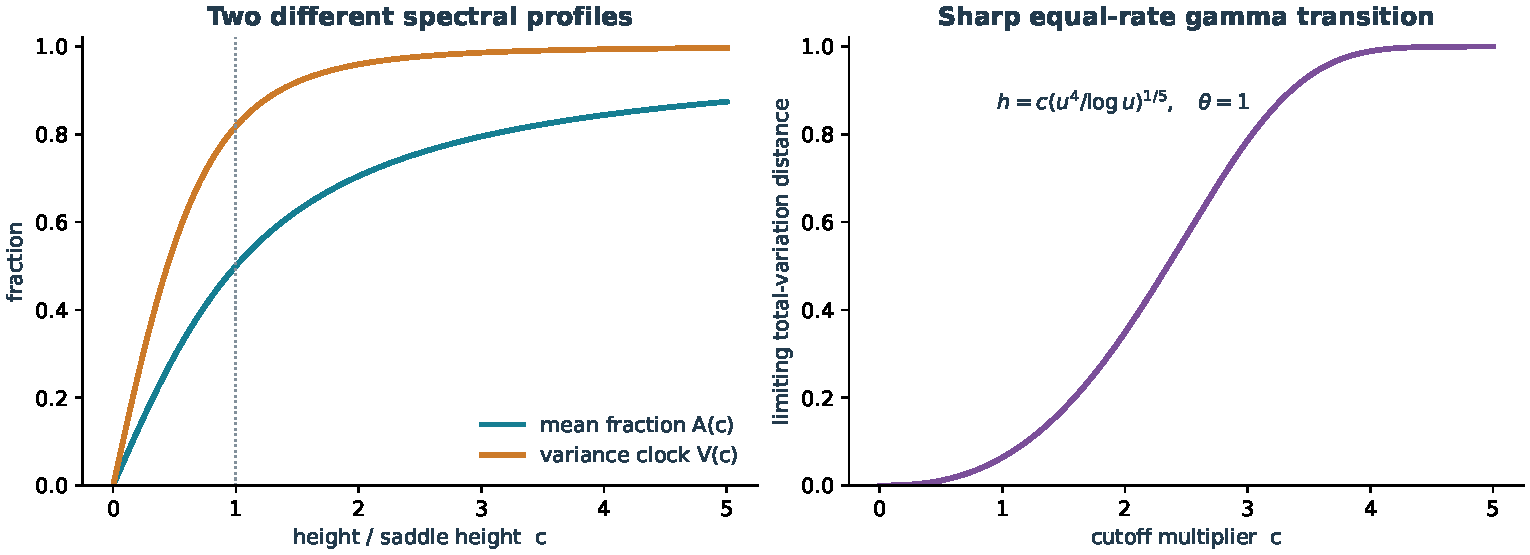
\includegraphics[width=\textwidth]{figures/universal_profiles.pdf}
 \caption{The mean allocation and fluctuation clock are different
 functions. The right panel shows the exact limiting distance in
 \eqref{eq:overview-TV}; these are analytic curves, not fitted data.}
 \label{fig:profiles}
\end{figure}

The proof also gives the conditional fraction contributed by ordinates
below $cu$:
\[
 \frac1X\sum_{\gamma_j\le cu}\frac{G_j}{\gamma_j^2}
 \longrightarrow A(c)=\frac2\pi\arctan c,
\]
uniformly in $c$ in probability. Thus half the contribution comes from
below the saddle height at first order. Its precise median height has a
systematic displacement of order $u/\log u$ and random fluctuations of
order $\sqrt{u/\log u}$. Section~\ref{sec:median} identifies both.

\subsection{What the source supplies}

The repository was pinned at commit
\texttt{2a9f8e3ee74a1824d57546f0b1b4f1cef5df93d6}.
Its vendored \texttt{Main.lean} exports Mathlib's ordinary
\texttt{RiemannHypothesis}, together with zero-free-half-plane and
critical-line theorems for Dirichlet $L$-functions~\cite{ProveItLean}.
The relevant GRH is the Dirichlet statement. A separate upstream
verification page reports kernel and external-checker verification of
the five theorem statements~\cite{Sutherland}.

The article's section \texttt{ana:sec:smalldev}, especially
\texttt{ana:thm:gammasum} and \texttt{ana:thm:smalldev}, supplies the
gamma series, its completed-function transform, and a detailed scalar
lower-tail asymptotic~\cite{ProveItArticle}. Its proof uses exponential
tilting and a local Gaussian limit for the total. The present work
extends that argument to independent spectral bands, to the exact
conditional density, and then to blocks whose dimension grows. The
arithmetic input is the completed-function identity and the classical
zero-counting formula. The new probability theorem is proved
independently under regular variation and does not use other unverified
claims from the merged article.

\subsection{Novelty and limits}

The reciprocal-$\xi$ law and the use of Hadamard products in probability
are established ideas~\cite{RoynetteYor,GaoHannigLeeTorcaso}. Conditioning
small Gaussian norms and conditional bridge limits for weighted sums
also have classical precedents~\cite{MayerWolfZeitouni,SobolevShklyaev}.
Sra's Appendix~C.17 contains a tilted Gaussian analysis for the
reciprocal-$\xi$ density~\cite{Sra}. We claim none of those mechanisms
as new.

The contribution developed here is the joint spectral conditional law,
the sharp growing-block total-variation transition and its explicit
four-fifths arithmetic specialization, the distinct macroscopic
independence transition, and the corrected median-height limit.
These results were not located in the inspected article or its seven
current incoming packets. The literature search found related general
conditioning results, but not these exact arithmetic statements. This
establishes a concrete extension of the supplied work; it does not
establish publication priority against all possible prior literature.

All new results have complete written proofs in this report. They have
not been formalized in Lean. The numerical artifacts illustrate finite
models and verify constants; they are not substitutes for the proofs.


% Standalone section for inclusion in the parent report.
% Required packages: amsmath, amssymb, amsthm, hyperref.
% The parent document supplies theorem, lemma, corollary, and remark environments.
% All proofs below are written independently; no part is a claimed Lean formalization.

\section{Conditioning a spectral gamma sum to be small}
\label{mc:sec:general}

The small-deviation result in the supplied article determines the probability
that a reciprocal-completed-$L$ random variable is very small.  We determine
the allocation of that small value among its spectral coordinates.  The
result has three scales: a deterministic allocation profile, Gaussian
fluctuations constrained by their total, and an exponential distance from
the conditioning boundary.  A second theorem gives a sharp threshold for
how many low spectral coordinates can simultaneously behave as independent
gamma variables.

The probabilistic statements hold for every regularly varying spectrum.
The role of RH or Dirichlet GRH in the application is to identify the
resulting probability law with the reciprocal of a completed $L$-function.
The general statements below require neither arithmetic input nor simple
spectral points.

\subsection{Definitions and main statement}

Let
\[
 0<\gamma_1\leq\gamma_2\leq\cdots,\qquad \gamma_j\longrightarrow\infty,
 \qquad N(T)=\#\{j:\gamma_j\leq T\},
\]
where repeated values are retained.  Assume that $N$ is regularly varying
with an index $\alpha>0$, meaning
\begin{equation}\label{mc:eq:RV}
 \frac{N(rT)}{N(T)}\longrightarrow r^\alpha
 \quad\text{for every }r>0\quad(T\longrightarrow\infty).
\end{equation}
Thus one may write $N(T)=T^\alpha L(T)$, with $L$ slowly varying;
a fixed positive constant may be absorbed into $L$.

Fix $p>\alpha$ and $\theta>0$.  Let $G_j$ be independent gamma variables
with shape $\theta$ and rate one, so their density is
$z^{\theta-1}e^{-z}/\Gamma(\theta)$ on $z>0$.  Define
\begin{equation}\label{mc:eq:XK}
 X=\sum_{j\geq1}\frac{G_j}{\gamma_j^p},\qquad
 K(t)=\theta\sum_{j\geq1}\log\left(1+\frac{t}{\gamma_j^p}\right).
\end{equation}
The series for $X$ converges almost surely and in $L^1$; in particular,
$\mathbb E e^{-tX}=e^{-K(t)}$ for $t\geq0$.

For $0<x<\mathbb E X$, let $t=t_x$ be the unique positive solution of
\begin{equation}\label{mc:eq:saddle}
 K'(t)=\theta\sum_j\frac{1}{\gamma_j^p+t}=x,
 \qquad u=t^{1/p}.
\end{equation}
Throughout, $x\downarrow0$, and hence $t,u\longrightarrow\infty$.
For $c\in[0,\infty]$, put
\begin{align}
 X_x(c)&=\sum_{\gamma_j\leq cu}\frac{G_j}{\gamma_j^p},
 &m_x(c)&=\theta\sum_{\gamma_j\leq cu}\frac{1}{\gamma_j^p+t},
 \label{mc:eq:partials}\\
 \sigma_x^2&=\theta\sum_j\frac{1}{(\gamma_j^p+t)^2},
 &Y_x&=t(x-X).
 \label{mc:eq:sigma}
\end{align}
At $c=\infty$ the sums run over every $j$, so $X_x(\infty)=X$ and
$m_x(\infty)=x$.  The deterministic centering in
\eqref{mc:eq:partials} is the \emph{exact tilted mean}; replacing it by only
its leading asymptotic is generally invalid on the fluctuation scale.

Write
\begin{align}
 C_1&=\int_0^\infty\frac{\alpha r^{\alpha-1}}{1+r^p}\,dr
     =\frac{\alpha\pi}{p\sin(\pi\alpha/p)},
 \label{mc:eq:C1}\\
 C_2&=\int_0^\infty\frac{\alpha r^{\alpha-1}}{(1+r^p)^2}\,dr
     =\left(1-\frac\alpha p\right)C_1,
 \label{mc:eq:C2}\\
 A(c)&=\frac1{C_1}\int_0^c\frac{\alpha r^{\alpha-1}}{1+r^p}\,dr,
 &V(c)&=\frac1{C_2}\int_0^c\frac{\alpha r^{\alpha-1}}{(1+r^p)^2}\,dr.
 \label{mc:eq:profiles}
\end{align}
Both $A$ and $V$ increase continuously from zero to one.  Let $B$ be a
standard Brownian bridge, that is, a centered Gaussian process with
\[
 \operatorname{Cov}(B(s),B(r))=\min(s,r)-sr,\qquad 0\leq s,r\leq1.
\]
For probability measures $P,Q$ on the same measurable space, use the
normalization
$d_{\mathrm{TV}}(P,Q)=\sup_E|P(E)-Q(E)|$; for densities this is one half
of their $L^1$ distance.

\begin{theorem}[Joint conditional spectral law]\label{mc:thm:joint}
Under the preceding assumptions:
\begin{enumerate}
\item The exact saddle and fluctuation size satisfy
\begin{equation}\label{mc:eq:scales}
 tx\sim\theta C_1N(u),\qquad
 t^2\sigma_x^2\sim\theta C_2N(u),\qquad
 \frac{\sigma_x}{x}\sim
 \frac{\sqrt{C_2}}{\sqrt\theta C_1\sqrt{N(u)}}.
\end{equation}

\item Fix $0<c_1<\cdots<c_k<\infty$ and an integer $m\geq0$.
Conditional on $X\leq x$, the vector
\begin{equation}\label{mc:eq:jointvector}
 \left(
 \left(\frac{X_x(c_i)-m_x(c_i)}{\sigma_x}\right)_{i=1}^k,
 Y_x,
 \left(\frac{tG_j}{\gamma_j^p}\right)_{j=1}^m
 \right)
\end{equation}
converges in total variation to
\begin{equation}\label{mc:eq:jointlimit}
 \left((B(V(c_i)))_{i=1}^k,\ E,\ (\Gamma_j)_{j=1}^m\right),
\end{equation}
where $E$ has the exponential distribution of rate one, the $\Gamma_j$
are independent gamma variables of shape $\theta$ and rate one, and these
three objects are mutually independent.

\item The allocation profile holds uniformly in the cutoff:
\begin{equation}\label{mc:eq:uniformLLN}
 \sup_{0\leq c\leq\infty}
 \left|\frac{X_x(c)}{x}-A(c)\right|
 \longrightarrow0
 \quad\text{in probability conditional on }X\leq x.
\end{equation}
The same conclusion holds with $X$ in place of $x$ in the denominator.
\end{enumerate}
\end{theorem}

The total-variation assertion is finite dimensional.  It is deliberately
stated only at finite positive cutoffs: the standardized value at
$c=\infty$ equals $-Y_x/(t\sigma_x)$, and a continuously distributed
variable cannot converge in total variation to the constant zero.  No
functional central limit theorem in a path space is asserted here.

\subsection{Summation over a regularly varying spectrum}

\begin{lemma}[Spectral sums]\label{mc:lem:sums}
If $q>\alpha/p$, then
\begin{equation}\label{mc:eq:spectral-sum}
 \frac1{N(u)}\sum_j\frac1{(1+(\gamma_j/u)^p)^q}
 \longrightarrow
 C_q:=\int_0^\infty\frac{\alpha r^{\alpha-1}}{(1+r^p)^q}\,dr.
\end{equation}
The analogous convergence holds when the sum and integral are restricted
to a fixed interval $(a,b]$ with $0\leq a<b\leq\infty$.
Moreover, $\sum_j\gamma_j^{-p}<\infty$, and, as $h\longrightarrow\infty$,
\begin{equation}\label{mc:eq:power-sum}
 \sum_{\gamma_j\leq h}\gamma_j^{2p}
 \sim\frac{\alpha}{\alpha+2p}\,h^{2p}N(h).
\end{equation}
\end{lemma}

\begin{proof}
The measures $N(u)^{-1}\sum_j\delta_{\gamma_j/u}$ converge on every
compact subinterval of $(0,\infty)$ to the measure
$\alpha r^{\alpha-1}\,dr$, by \eqref{mc:eq:RV} and approximation of
continuous functions by step functions.  There is no difficulty at zero:
the integrand in \eqref{mc:eq:spectral-sum} is at most one, and the mass
below $\delta$ has limit $\delta^\alpha$.

For completeness, the required uniform control at infinity follows
directly from dyadic ratios.  Given $\varepsilon>0$, regular variation
implies
\[
 \frac{N(2T)}{N(T)}\leq2^{\alpha+\varepsilon}
 \quad(T\geq T_0).
\]
Iterating and using monotonicity gives, for $u\geq T_0$ and $r\geq1$,
$N(ru)/N(u)\leq C_\varepsilon r^{\alpha+\varepsilon}$.
Choose $0<\varepsilon<pq-\alpha$.  The part with $\gamma_j/u>R\geq1$
is at most
\[
 C\sum_{\ell\geq0}(2^\ell R)^{-pq}
                  (2^{\ell+1}R)^{\alpha+\varepsilon},
\]
which tends to zero as $R\to\infty$, uniformly in large $u$.
This proves the sum limit and its interval version.  The same dyadic
estimate, with an exponent between $\alpha$ and $p$, proves
$\sum_j\gamma_j^{-p}<\infty$.

Finally, Stieltjes integration by parts gives
\[
 \sum_{\gamma_j\leq h}\gamma_j^{2p}
 =h^{2p}N(h)-2p\int_0^h r^{2p-1}N(r)\,dr.
\]
After division by $h^{2p}N(h)$, dominated convergence applies to the
integral on $[0,1]$: $N(hs)/N(h)\leq1$ there and tends to $s^\alpha$.
The resulting limit is
$1-2p/(\alpha+2p)=\alpha/(\alpha+2p)$.
The constants \eqref{mc:eq:C1}--\eqref{mc:eq:C2} follow from the beta
integral after substituting $s=r^p$.
\end{proof}

\subsection{Tilting and a uniform local limit}

Since $\mathbb EX=\theta\sum_j\gamma_j^{-p}<\infty$, the nonnegative
series defining $X$ is finite almost surely.  Its Laplace transform in
\eqref{mc:eq:XK} follows by monotone convergence of the partial sums and
the gamma Laplace transform.  Termwise differentiation is justified on
every compact set of $t\geq0$.  The function $K'$ is continuous, strictly
decreasing from $\mathbb EX$ to zero, proving existence and uniqueness of
\eqref{mc:eq:saddle}.  The event $X\leq x$ has positive probability for
every $x>0$: choose a finite initial segment with expected remaining tail
less than $x/4$, apply Markov's inequality to the tail, and require each
of the finitely many initial summands to be sufficiently small.

Introduce the tilted probability measure
\begin{equation}\label{mc:eq:tilt}
 d\mathbb P_t=e^{-tX+K(t)}\,d\mathbb P.
\end{equation}
Under $\mathbb P_t$, the variables
$\widetilde G_j=(1+t/\gamma_j^p)G_j$ are independent gamma variables
of shape $\theta$ and rate one.  Indeed, the assertion follows first for
every finite group of coordinates by integrating out its independent
tail, and those finite-dimensional identities characterize the product
law.  Set
\begin{equation}\label{mc:eq:av}
 a_j=\frac{t}{\gamma_j^p+t}
     =\frac1{1+(\gamma_j/u)^p},\qquad
 v=\theta\sum_j a_j^2=t^2\sigma_x^2,
 \qquad S=tX=\sum_j a_j\widetilde G_j.
\end{equation}
The mean of $S$ under $\mathbb P_t$ is $tx$, and its variance is $v$.
Lemma~\ref{mc:lem:sums} gives \eqref{mc:eq:scales} and $v\to\infty$.

\begin{lemma}[Uniform local Gaussian limit on a spectral band]
\label{mc:lem:local}
Let $I=(a,b]\subset(0,\infty)$, with $0\leq a<b\leq\infty$.
Delete any fixed finite set of indices if desired, and write
\[
 Z_{I,u}=\frac1{\sqrt v}
 \sum_{\gamma_j/u\in I}a_j(\widetilde G_j-\theta).
\]
For all sufficiently large $u$, this variable has a continuous density
$f_{I,u}$, and
\begin{equation}\label{mc:eq:local}
 \sup_z|f_{I,u}(z)-\varphi_{\lambda_I}(z)|\longrightarrow0,
 \qquad
 \int_{\mathbb R}|f_{I,u}-\varphi_{\lambda_I}|\longrightarrow0,
\end{equation}
where $\varphi_\lambda$ is the centered normal density of variance
\[
 \lambda_I=\frac1{C_2}
 \int_I\frac{\alpha r^{\alpha-1}}{(1+r^p)^2}\,dr>0.
\]
The same conclusion holds for the whole spectrum with any lower block
$\{\gamma_j\leq h(u)\}$ removed, provided $h(u)=o(u)$; its limiting
variance is then one.
\end{lemma}

\begin{proof}
For a band, Lemma~\ref{mc:lem:sums} gives
$\theta\sum_Ia_j^2/v\to\lambda_I$.  For a fixed Fourier variable $z$,
the logarithm of the centered characteristic function is
\begin{align*}
 \log\phi_{I,u}(z)
 &=\theta\sum_I\left[-\frac{iza_j}{\sqrt v}
              -\log\left(1-\frac{iza_j}{\sqrt v}\right)\right]\\
 &=-\frac{\theta z^2}{2v}\sum_Ia_j^2
     +O_\theta\left(\frac{|z|^3\sum_Ia_j^3}{v^{3/2}}\right)
 \longrightarrow-\lambda_Iz^2/2.
\end{align*}
Here $0<a_j\leq1$, so the remainder is $O_z(v^{-1/2})$.

We now prove the Fourier integrability needed for a local, rather than
merely weak, limit.  Choose a compact interval $[a',b']$ strictly inside
$I$ with $0<a'<b'<\infty$.  There are at least $dN(u)$ spectral indices
in this interval for all large $u$, each with
$a_j\geq(1+(b')^p)^{-1}$.  Since $v\asymp N(u)$,
\begin{equation}\label{mc:eq:fourier-envelope}
 |\phi_{I,u}(z)|
 =\prod_I\left(1+\frac{z^2a_j^2}{v}\right)^{-\theta/2}
 \leq\left(1+\frac{Az^2}{N(u)}\right)^{-DN(u)}
\end{equation}
for constants $A,D>0$.  A finite deletion does not change this estimate.
Write $n=N(u)$.  For $|z|\leq\sqrt n$, the right side is at most
$\exp(-ADz^2/(1+A))$.  For the remaining tail,
\begin{align*}
 \int_{\sqrt n}^\infty
     \left(1+\frac{Az^2}{n}\right)^{-Dn}\,dz
 &=\sqrt n\int_1^\infty(1+Ar^2)^{-Dn}\,dr\\
 &\leq C\sqrt n(1+A)^{-Dn/2}\longrightarrow0,
\end{align*}
where, for large $n$, the remaining half of the power is bounded by
$(1+Ar^2)^{-1}$.  These estimates show uniform integrability of the
characteristic functions and convergence in $L^1$ to
$e^{-\lambda_Iz^2/2}$.  Fourier inversion proves uniform convergence of
the densities.  Their $L^1$ convergence follows from pointwise
convergence and equality of their integrals to one (Scheff\'e's lemma).

For a deleted lower block, $N(h)/N(u)\to0$.  To see this without any
uniform regular-variation theorem, fix $\delta>0$ and use
$h\leq\delta u$ eventually, so
$\limsup N(h)/N(u)\leq\delta^\alpha$, then let $\delta\downarrow0$.
The removed variance is at most $\theta N(h)=o(v)$.  The interval
$[u,2u]$ remains available for the Fourier envelope, and the same proof
applies with limiting variance one.
\end{proof}

\subsection{Proof of the joint conditional law}

\begin{proof}[Proof of Theorem~\ref{mc:thm:joint}]
Only the conditional conclusions remain.  Under $\mathbb P_t$, put
\[
 W=\frac{tX-tx}{\sqrt v},\qquad
 D_u=\mathbb E_t\bigl[e^{\sqrt vW}\mathbf1_{\{W\leq0\}}\bigr].
\]
The density $f_u$ of $W$ satisfies Lemma~\ref{mc:lem:local} with
limiting variance one.  On writing $y=-\sqrt vW$, we obtain
\begin{equation}\label{mc:eq:D}
 \sqrt vD_u=\int_0^\infty e^{-y}f_u(-y/\sqrt v)\,dy
 \longrightarrow\varphi_1(0)=\frac1{\sqrt{2\pi}}.
\end{equation}
The density of $\mathbb P(\,\cdot\mid X\leq x)$ with respect to
$\mathbb P_t$ is exactly
\begin{equation}\label{mc:eq:condition-weight}
 D_u^{-1}e^{\sqrt vW}\mathbf1_{\{W\leq0\}}.
\end{equation}

First omit the $m$ specified low coordinates.  Partition the remaining
indices into the $k+1$ bands
\[
 I_1=(0,c_1],\ I_2=(c_1,c_2],\ldots,
 I_k=(c_{k-1},c_k],\ I_{k+1}=(c_k,\infty).
\]
For large $u$, all $m$ omitted indices belong to $I_1$.
The centered sums on these bands, divided by $\sqrt v$, have independent
densities $f_{i,u}$ from Lemma~\ref{mc:lem:local}.  Their limiting
variances are
\[
 \lambda_i=V(c_i)-V(c_{i-1})\quad(1\leq i\leq k),
 \qquad \lambda_{k+1}=1-V(c_k),\qquad c_0=0.
\]
Let $U_i$ denote the standardized increment on the \emph{full} band
$I_i$, including the omitted coordinates if $i=1$.  For specified values
$r=(r_1,\ldots,r_m)>0$ of the scaled low coordinates
$tG_j/\gamma_j^p=a_j\widetilde G_j$, put
\[
 \delta_u(r)=\frac1{\sqrt v}\sum_{j=1}^m(r_j-\theta a_j).
\]
Under the tilted measure their joint density is
\[
 q_u(r)=\prod_{j=1}^m
 \frac{r_j^{\theta-1}e^{-r_j/a_j}}
      {\Gamma(\theta)a_j^\theta}.
\]
For fixed $r>0$, $q_u(r)$ tends to the product $q(r)$ of unit-rate gamma
densities, and $\delta_u(r)\to0$.

Transform the last band increment to $y=-\sqrt v\sum_{i=1}^{k+1}U_i$.
The Jacobian is $1/\sqrt v$.  Equations
\eqref{mc:eq:condition-weight} and \eqref{mc:eq:D} show that the joint
conditional density of $(U_1,\ldots,U_k,Y_x,r)$ is
\begin{equation}\label{mc:eq:jointdensity}
 \frac{e^{-y}\mathbf1_{\{y\geq0\}}q_u(r)}{\sqrt vD_u}
 f_{1,u}(z_1-\delta_u(r))
 \prod_{i=2}^k f_{i,u}(z_i)
 f_{k+1,u}\left(-\frac{y}{\sqrt v}-\sum_{i=1}^kz_i\right).
\end{equation}
For almost every fixed $(z,y,r)$, this converges to
\begin{equation}\label{mc:eq:limitdensity}
 \frac{e^{-y}\mathbf1_{\{y\geq0\}}q(r)}{\varphi_1(0)}
 \prod_{i=1}^k\varphi_{\lambda_i}(z_i)
 \varphi_{\lambda_{k+1}}\left(-\sum_{i=1}^kz_i\right).
\end{equation}
The product of normal densities in \eqref{mc:eq:limitdensity}, divided
by $\varphi_1(0)$, integrates to one: it is the conditional density of
independent centered normal increments of variances $\lambda_i$ given
that their sum is zero.  Consequently the entire limiting density
integrates to one.  Scheff\'e's lemma now gives total-variation
convergence of \eqref{mc:eq:jointdensity} to
\eqref{mc:eq:limitdensity}.

The cumulative increments have covariance
\[
 \sum_{i\leq\min(a,b)}\lambda_i
 -\left(\sum_{i\leq a}\lambda_i\right)
  \left(\sum_{i\leq b}\lambda_i\right)
 =V(\min(c_a,c_b))-V(c_a)V(c_b).
\]
Their distribution is therefore that of $(B(V(c_i)))_{i=1}^k$.
An invertible linear cumulative-sum transformation preserves total
variation, and the factorization in \eqref{mc:eq:limitdensity} proves
all the independence assertions.

For the uniform law of large numbers, Lemma~\ref{mc:lem:sums} gives
$m_x(c)/x\to A(c)$ for every finite $c$, while
\eqref{mc:eq:scales} gives $\sigma_x/x\to0$.  The finite-dimensional
limit therefore implies $X_x(c)/x\to A(c)$ in conditional probability
at every finite positive $c$.  At infinity,
\[
 \frac Xx=1-\frac{Y_x}{tx}\longrightarrow1,
\]
because $Y_x$ is tight and $tx\to\infty$.  Choose a finite grid of
cutoffs, including infinity, on which consecutive values of the
continuous function $A$ differ by at most $\varepsilon$.  Monotonicity
of $X_x(c)$ brackets every intermediate value between its two grid
values.  A union bound at the finitely many endpoints proves
\eqref{mc:eq:uniformLLN}.  Finally $X/x\to1$, so division by $X$ gives
the same uniform limit.
\end{proof}

\section{A sharp threshold for simultaneous gamma equilibration}
\label{mc:sec:threshold}

The fixed-coordinate conclusion of Theorem~\ref{mc:thm:joint} does not
specify how many coordinates may be treated as independent at once.
The next theorem gives an exact asymptotic answer in total-variation
distance.

Let $h=h(u)>0$ satisfy $h=o(u)$, and define the finite lower block
\[
 J_u=\{j:\gamma_j\leq h\},\qquad
 s_j=(\gamma_j/u)^p\quad(j\in J_u),\qquad
 \tau_u^2=\theta\sum_{j\in J_u}s_j^2
          =\frac\theta{u^{2p}}
            \sum_{\gamma_j\leq h}\gamma_j^{2p}.
\]
Let $Q_u$ be the conditional law of
$(tG_j/\gamma_j^p)_{j\in J_u}$ given $X\leq x$.  On the same
finite-dimensional space put
\[
 P_u=\bigotimes_{j\in J_u}\operatorname{Gamma}(\theta,1+s_j),
 \qquad
 R_u=\bigotimes_{j\in J_u}\operatorname{Gamma}(\theta,1),
\]
where the second gamma parameter is the rate.  Empty products have
their usual one-point interpretation.

\begin{theorem}[Sharp growing-block law]\label{mc:thm:threshold}
For every $h(u)=o(u)$:
\begin{enumerate}
\item The conditioning is asymptotically equivalent, on the whole
growing block, to independent exponential tilting:
\begin{equation}\label{mc:eq:canonical}
 d_{\mathrm{TV}}(Q_u,P_u)\longrightarrow0.
\end{equation}
More strongly, the joint conditional law of the block and $Y_x$ is
at total-variation distance tending to zero from
$P_u\otimes\operatorname{Exp}(1)$.

\item If $\Phi$ is the standard normal distribution function, then
\begin{equation}\label{mc:eq:sharpTV}
 d_{\mathrm{TV}}(Q_u,R_u)
 =2\Phi(\tau_u/2)-1+o(1).
\end{equation}
In particular, convergence to independent unit-rate gamma coordinates
holds if and only if $\tau_u\to0$.  If $\tau_u\to\tau\in(0,\infty)$,
the limiting distance is $2\Phi(\tau/2)-1$; if $\tau_u\to\infty$, the
distance tends to one.  The same asymptotic distance holds when the
boundary slack is included and compared with an independent
$\operatorname{Exp}(1)$ variable.

\item When $h\to\infty$, the threshold parameter has the spectral form
\begin{equation}\label{mc:eq:tauRV}
 \tau_u^2\sim
 \frac{\theta\alpha}{\alpha+2p}\,
 N(h)\left(\frac hu\right)^{2p}.
\end{equation}
\end{enumerate}
\end{theorem}

\begin{proof}
\emph{Conditioning versus tilting.}
Work under $\mathbb P_t$.  With $S=tX$ from \eqref{mc:eq:av}, write
$S=S_B+S_R$ for the lower block and its independent remainder, and let
$\mu_B,\mu_R$ be their means.  Thus $\mu_B+\mu_R=tx$.
The distribution of the block under $\mathbb P_t$ is exactly $P_u$.
Moreover,
\[
 \operatorname{Var}_t(S_B)=\theta\sum_{J_u}a_j^2
 \leq\theta N(h)=o(v).
\]
By Lemma~\ref{mc:lem:local}, the density $g_u$ of
$(S_R-\mu_R)/\sqrt v$ converges uniformly to $\varphi_1$, and is
uniformly bounded for all large $u$.

Relative to $P_u\otimes\operatorname{Exp}(1)$, the joint conditional
law of the block values $r=(r_j)_{j\in J_u}$ and the boundary slack $y$
has the exact density
\begin{equation}\label{mc:eq:blockratio}
 L_u(r,y)=\frac1{\sqrt vD_u}
 g_u\left(-\frac{\sum_{j\in J_u}r_j-\mu_B+y}{\sqrt v}\right).
\end{equation}
Indeed, after fixing the block, the remainder must have value
$tx-\sum r_j-y$, and the same change of variables as before supplies
the Jacobian $1/\sqrt v$ and the factor $e^{-y}$.
Under the reference measure in \eqref{mc:eq:blockratio},
\[
 \frac{\sum r_j-\mu_B+y}{\sqrt v}\longrightarrow0
 \quad\text{in probability},
\]
by the variance estimate and the exponential law of $y$.
Uniform convergence of $g_u$ and \eqref{mc:eq:D} imply
$L_u\to1$ in probability.  The same estimates bound $L_u$ uniformly,
so $\mathbb E|L_u-1|\to0$.  This proves the joint assertion and its
marginal \eqref{mc:eq:canonical}.

\emph{The exact statistical transition.}
Under $R_u$, let $Z_j$ be its independent unit-rate gamma coordinates.
The log likelihood of $P_u$ relative to $R_u$ is
\begin{equation}\label{mc:eq:LAN}
 \ell_u=\sum_{J_u}\{\theta\log(1+s_j)-s_jZ_j\}.
\end{equation}
Since $\max_{J_u}s_j\leq(h/u)^p\to0$,
\begin{align*}
 \mathbb E_{R_u}\ell_u
   &=-\frac{\tau_u^2}{2}
     +O\left(\max_{J_u}s_j\,\tau_u^2\right),\\
 \operatorname{Var}_{R_u}(\ell_u)&=\tau_u^2.
\end{align*}
If $\tau_u\to\tau\in(0,\infty)$, the Lyapunov estimate
\[
 \sum_{J_u}\mathbb E|s_j(Z_j-\theta)|^3
 \leq C_\theta\max_{J_u}s_j\sum_{J_u}s_j^2\longrightarrow0
\]
proves
$\ell_u\Rightarrow\mathcal N(-\tau^2/2,\tau^2)$.
For $\tau=0$, the same conclusion with a point mass at zero follows
directly from the first two moments.
The identity
\[
 d_{\mathrm{TV}}(P_u,R_u)
 =\mathbb E_{R_u}(1-e^{\ell_u})_+
\]
involves a bounded continuous function of $\ell_u$.  Hence, for finite
$\tau$, the limiting distance is
\begin{align*}
 \mathbb E(1-e^Z)_+
 &=\Phi(\tau/2)-\Phi(-\tau/2)\\
 &=2\Phi(\tau/2)-1,
 \qquad Z\sim\mathcal N(-\tau^2/2,\tau^2).
\end{align*}

If $\tau_u\to\infty$, the Hellinger affinity is explicit:
\begin{equation}\label{mc:eq:affinity}
 \int\sqrt{dP_u\,dR_u}
 =\prod_{J_u}\left(\frac{2\sqrt{1+s_j}}{2+s_j}\right)^\theta,
 \qquad
 \log\int\sqrt{dP_u\,dR_u}
 =-\frac{\tau_u^2}{8}(1+o(1)).
\end{equation}
It tends to zero.  Since
$1-d_{\mathrm{TV}}(P_u,R_u)=\int\min(dP_u,dR_u)$ is at most this
affinity, the total-variation distance tends to one.

Every sequence of $\tau_u\in[0,\infty)$ has a subsequence converging
in $[0,\infty]$.  The preceding arguments on each such subsequence
give the full asymptotic formula
$d_{\mathrm{TV}}(P_u,R_u)=2\Phi(\tau_u/2)-1+o(1)$, even when
$\tau_u$ has no limit.  The triangle inequality and
\eqref{mc:eq:canonical} give \eqref{mc:eq:sharpTV}.  Tensoring both
measures with the same exponential law preserves total variation,
which proves the statement about the slack.  Finally,
\eqref{mc:eq:tauRV} is exactly \eqref{mc:eq:power-sum}.
\end{proof}

\subsection{The larger threshold for independence with unequal rates}

Unit-rate equilibration and independence with the correct unequal rates
have different ranges.  To describe the latter, drop the restriction
$h=o(u)$ and retain the definitions of $Q_u$ and $P_u$ for an arbitrary
positive cutoff $h=h(u)$.  Define
\begin{equation}\label{mc:eq:Dprofile}
 \mathcal D(\rho)=2\left[
 \Phi\left(\sqrt{\frac{-\log(1-\rho)}{\rho}}\right)
 -\Phi\left(\sqrt{
       \frac{-(1-\rho)\log(1-\rho)}{\rho}}\right)\right],
 \qquad 0<\rho<1,
\end{equation}
and extend it continuously by $\mathcal D(0)=0$ and
$\mathcal D(1)=1$.

\begin{theorem}[Sharp boundary for independent tilted coordinates]
\label{mc:thm:macroscopic}
For every positive cutoff function $h(u)$,
\begin{equation}\label{mc:eq:macroTV}
 d_{\mathrm{TV}}(Q_u,P_u)
 =\mathcal D\bigl(V(h/u)\bigr)+o(1).
\end{equation}
Consequently, $d_{\mathrm{TV}}(Q_u,P_u)\to0$ if and only if $h=o(u)$.
If $h/u\to c\in(0,\infty)$, its limit is the strictly positive number
$\mathcal D(V(c))$; if $h/u\to\infty$, its limit is one.
\end{theorem}

\begin{proof}
Suppose first that $h/u\to c\in(0,\infty)$ and put $\rho=V(c)$.
The sum lemma and the local limit lemma apply to the moving cutoff:
the limiting variances follow by bracketing $h/u$ between $c-\varepsilon$
and $c+\varepsilon$, and fixed compact interior intervals still supply
the Fourier envelopes.  Therefore, under $P_u$, the centered block sum
\[
 Z_u=(S_B-\mu_B)/\sqrt v
\]
converges in distribution to $Z\sim\mathcal N(0,\rho)$, while the
remainder density $g_u$ converges uniformly to
$\varphi_{1-\rho}$.  Integrating \eqref{mc:eq:blockratio} over the
exponential slack shows that the marginal likelihood of $Q_u$
relative to $P_u$ differs, uniformly in the block values, by $o(1)$
from
\[
 r(Z_u)=\frac{\varphi_{1-\rho}(-Z_u)}{\varphi_1(0)}
       =(1-\rho)^{-1/2}
         \exp\left(-\frac{Z_u^2}{2(1-\rho)}\right).
\]
Uniformity follows from uniform convergence of $g_u$,
\eqref{mc:eq:D}, and the bounded derivative of the limiting normal
density: the additional shift $y/\sqrt v$ has average $1/\sqrt v$
under the exponential law.  The function $r$ is bounded and
continuous.  Thus
\[
 d_{\mathrm{TV}}(Q_u,P_u)
 \longrightarrow\tfrac12\mathbb E|r(Z)-1|.
\]
Multiplying the density of $\mathcal N(0,\rho)$ by $r$ gives the
density of $\mathcal N(0,\rho(1-\rho))$.  Their densities cross at
\[
 |z|=\sqrt{-(1-\rho)\log(1-\rho)}.
\]
Integrating the difference on the interval between these crossing
points gives precisely \eqref{mc:eq:Dprofile}.

The case $h/u\to0$ is Theorem~\ref{mc:thm:threshold}.
If $h/u\to\infty$, restrict to the smaller block with cutoff $bu$
for a fixed $b>0$.  Total variation cannot increase under this
marginalization, so
\[
 \liminf d_{\mathrm{TV}}(Q_u,P_u)\geq\mathcal D(V(b)).
\]
Letting $b\to\infty$ makes the right side tend to one.
The formula for an arbitrary $h/u$ now follows by taking subsequences
in the compactified interval $[0,\infty]$.  The claimed equivalence
uses that $V(c)>0$ and $\mathcal D(V(c))>0$ for every $c>0$.
\end{proof}

\subsection{The explicit transition for the reciprocal-$\xi$ law}

For the positive ordinates of Riemann zeros, counted with multiplicity,
$N(T)\sim T\log T/(2\pi)$.  Taking $p=2$ gives $\alpha=1$,
$C_1=\pi/2$, and $C_2=\pi/4$.  Consequently
\begin{equation}\label{mc:eq:riemannprofiles}
 A(c)=\frac2\pi\arctan c,
 \qquad
 V(c)=\frac2\pi\left(\arctan c+\frac{c}{1+c^2}\right),
\end{equation}
and, in the last equivalence below, assuming $h\to\infty$,
\begin{equation}\label{mc:eq:riemannscales}
 x\sim\frac{\theta\log u}{4u},\qquad
 \sigma_x^2\sim\frac{\theta\log u}{8u^3},\qquad
 \tau_u^2\sim\frac{\theta h^5\log h}{10\pi u^4}.
\end{equation}
These same leading formulas hold for a fixed primitive real Dirichlet
character, with central zeros omitted.

In particular, if
\begin{equation}\label{mc:eq:criticalheight}
 h=c\left(\frac{u^4}{\log u}\right)^{1/5},\qquad c>0,
\end{equation}
then the total-variation distance from independent unit-rate gamma
coordinates has the explicit limit
\begin{equation}\label{mc:eq:criticalTV}
 2\Phi\left(\frac12\sqrt{\frac{2\theta c^5}{25\pi}}\right)-1.
\end{equation}
If $h$ is smaller than the scale in \eqref{mc:eq:criticalheight} by a
factor tending to zero, that distance tends to zero.  If it is larger
by a factor tending to infinity, the distance tends to one, with no
additional restriction on $h/u$.  Indeed, in the latter case restrict
to the subblock with cutoff
\[
 h'=\min(h,u/\log u).
\]
Then $h'=o(u)$ and $h'/(u^4/\log u)^{1/5}\to\infty$, so
Theorem~\ref{mc:thm:threshold} gives distance tending to one for the
subblock; marginalization gives the same lower bound for the full
block.  Thus \eqref{mc:eq:criticalTV}, with its continuous endpoint
values zero and one at $c=0$ and $c=\infty$, describes every limiting
ratio $h/(u^4/\log u)^{1/5}\to c\in[0,\infty]$.

The fifth power and the logarithmic correction are
forced by the accumulated rate discrepancy across the growing block,
not by a bound on any single coordinate.  This threshold is smaller
than the scale $h\asymp u$ in Theorem~\ref{mc:thm:macroscopic}, where
the conditioning creates a nonvanishing dependence even after the
correct unequal rates are retained.

Under RH, the paired Hadamard product supplies the arithmetic identity
\begin{equation}\label{mc:eq:xilaw}
 \mathbb E e^{-tX}
 =\left(\frac{\xi(1/2)}{\xi(1/2+\sqrt t)}\right)^\theta.
\end{equation}
This is the precise bridge from the supplied article's gamma law to
the conditional theorems proved here.  The general probability theorem is
independent of RH; identification \eqref{mc:eq:xilaw} is where RH
enters.  It makes no assertion about simple zeros, zero correlations,
or unproved linear independence of ordinates.

\subsection{Complex characters and finite products}

The construction also covers a primitive nonreal Dirichlet character
$\chi$, by pairing it with its conjugate.  With its usual completed
function $\Lambda_\chi$ and central order
$m=\operatorname{ord}_{s=1/2}\Lambda_\chi(s)$, put
\begin{equation}\label{mc:eq:complexproduct}
 H_\chi(w)=
 \frac{\Lambda_\chi(1/2+w)\Lambda_{\bar\chi}(1/2+w)}{w^{2m}},
\end{equation}
with the removable singularity at zero filled in.  The functional
equations make $H_\chi$ even.  On the real axis the numerator is
$|\Lambda_\chi(1/2+w)|^2$, so
\[
 H_\chi(0)=\left|\frac{\Lambda_\chi^{(m)}(1/2)}{m!}\right|^2>0.
\]
Under Dirichlet GRH, the paired Hadamard factorization gives
\[
 \frac{H_\chi(w)}{H_\chi(0)}
 =\prod_{\gamma_j>0}\left(1+\frac{w^2}{\gamma_j^2}\right),
\]
where the positive zeros of the two completed functions are combined,
retaining their multiplicities.  The product converges locally
uniformly because $\sum_j\gamma_j^{-2}<\infty$.  Evenness eliminates
the linear exponential factor in the order-one Hadamard product.
Thus the gamma sum has Laplace transform
\[
 \mathbb E e^{-tX}
 =\left(\frac{H_\chi(0)}{H_\chi(\sqrt t)}\right)^\theta.
\]
Its positive spectral count satisfies
$N(T)\sim2T\log T/(2\pi)$.

More generally, multiply finitely many such conjugate-pair factors,
real primitive Dirichlet factors with their central powers removed,
and copies of $\xi(1/2+w)$.  If $d$ is the number of degree-one
completed factors before conjugate pairing, the positive spectrum has
\[
 N(T)\sim\frac{d}{2\pi}T\log T.
\]
The profiles $A$ and $V$ in \eqref{mc:eq:riemannprofiles} are unchanged.
The first two equivalents in \eqref{mc:eq:riemannscales} acquire a
factor $d$, and the threshold parameter becomes
\[
 \tau_u^2\sim\frac{\theta d\,h^5\log h}{10\pi u^4}
 \qquad(h\to\infty).
\]
At the critical height \eqref{mc:eq:criticalheight}, the limiting
distance from independent unit-rate gamma coordinates is therefore
\begin{equation}\label{mc:eq:degreeprofile}
 2\Phi\left(c^{5/2}\sqrt{\frac{\theta d}{50\pi}}\right)-1.
\end{equation}
The leading transition depends only on the total degree and the gamma
shape.  The conductors, root numbers, locations of individual zeros,
and their multiplicities affect the exact saddle and finite-scale
corrections, but not this limiting profile.

\begin{corollary}[The sharp exponent in the number of coordinates]
\label{mc:cor:four-fifths}
For any fixed degree $d$ in the preceding construction, write
$n=N(u)$ and $k=N(h)$.  If
\[
 \frac{k}{n^{4/5}}\longrightarrow\kappa\in[0,\infty],
\]
then the total-variation distance from $k$ independent unit-rate gamma
coordinates tends to
\begin{equation}\label{mc:eq:countprofile}
 2\Phi\left(\frac12\sqrt{\frac{125\theta}{256}\,\kappa^5}\right)-1,
\end{equation}
with value one at $\kappa=\infty$.  In particular, unit-rate
equilibration holds for $k=o(n^{4/5})$, and fails maximally when
$k/n^{4/5}\to\infty$.  Independence with the correct unequal rates
holds on the larger range $k=o(n)$.
\end{corollary}

\begin{proof}
At $h=c(u^4/\log u)^{1/5}$, the counting asymptotic gives
\[
 \frac{N(h)}{N(u)^{4/5}}
 \longrightarrow\frac{4c}{5}
                     \left(\frac d{2\pi}\right)^{1/5}.
\]
Substitute
$c=(5\kappa/4)(2\pi/d)^{1/5}$ into
\eqref{mc:eq:degreeprofile}; the degree cancels and
$\tau^2=125\theta\kappa^5/256$.
Monotonicity of the count brackets any sequence with a finite positive
limiting ratio between such critical cutoffs.  The zero and infinity
cases follow by the same bracketing and marginalization.  Finally,
regular variation implies $N(h)/N(u)\to0$ if and only if $h/u\to0$,
so Theorem~\ref{mc:thm:macroscopic} gives the last assertion.
\end{proof}

% Suggested bibliography keys/entries for the parent report:
% Article: pinned ProveIt Article/sections/ana.tex, blob
% 6b414e43f44bd89c5a7fce0c0f2a0cf08626cc8b, specifically
% ana:thm:gammasum and ana:thm:smalldev, lines 2955--3057.
% CampenhoutCover1981: Jan M. van Campenhout and Thomas M. Cover,
% Maximum Entropy and Conditional Probability, IEEE Trans. Inform. Theory
% IT-27 (1981), no.4, 483--489.
% https://isl.stanford.edu/people/cover/papers/transIT/0483camp.pdf
% MayerWolfZeitouni1993: Eddy Mayer-Wolf and Ofer Zeitouni,
% The Probability of Small Gaussian Ellipsoids and Associated Conditional
% Moments, Ann. Probab. 21 (1993), no.1, 14--24.
% https://doi.org/10.1214/aop/1176989391
% Author preprint: https://www.wisdom.weizmann.ac.il/~zeitouni/pdf/eddyelip.pdf

\section{Explicit centering and the height carrying half the total}
\label{sec:median}

We now specialize to the positive noncentral zero ordinates of $\zeta$
or of a fixed primitive real Dirichlet character $\chi$. For $\zeta$ put
$q=1$; otherwise $q$ is the conductor. Keep a fixed $\theta>0$.
Every occurrence of a zero is counted, so a zero of multiplicity $m$
contributes $m$ independent shape-$\theta$ variables, equivalently one
shape-$m\theta$ variable. A possible central zero is excluded from the
series and removed from the completed-function product.

The positive-ordinate counting formula is
\begin{equation}\label{med:eq:count}
 N(T)=\frac{T}{2\pi}\left(\log\frac{qT}{2\pi}-1\right)
       +O_\chi(\log(T+2)).
\end{equation}
For real characters this is half the usual both-sign count, up to the
finite central multiplicity; see~\cite{BennettEtAl}. For $\zeta$ it is
the Riemann--von Mangoldt formula. All constants below may depend on the
fixed function and on $\theta$.

Let $u$ be the exact saddle from \eqref{mc:eq:saddle} with $p=2$, and set
\[
 \ell=\log\frac{qu}{2\pi},\qquad
 J(c)=\int_0^c\frac{\log r}{1+r^2}\,dr,\qquad
 M_u(c)=\frac{\theta}{2\pi u}
                 \bigl(\ell\arctan c+J(c)\bigr).
\]
The first correction $J$ matters: $J(1)=-G$, where
$G=\sum_{n\ge0}(-1)^n/(2n+1)^2$ is Catalan's constant.

\begin{lemma}[Centering accurate on the fluctuation scale]
\label{med:lem:center}
Uniformly for $c$ in any compact subset of $(0,\infty)$,
\begin{align}
 m_x(c)&=M_u(c)+O_\chi\left(\frac{\log u}{u^2}\right)
                  =M_u(c)+o(\sigma_x),\label{med:eq:mean}\\
 x&=\frac{\theta\ell}{4u}
                  +O_\chi\left(\frac{\log u}{u^2}\right),\label{med:eq:total}\\
 \sigma_x^2&=\frac{\theta(\ell-1)}{8u^3}
                  +O_\chi\left(\frac{\log u}{u^4}\right).
                  \label{med:eq:variance}
\end{align}
\end{lemma}

\begin{proof}
Write the error in \eqref{med:eq:count} as $R(T)$, extending the formula
to $T\ge0$ by increasing its constant; then $R(0)=0$. Stieltjes
integration by parts with $f(T)=(T^2+u^2)^{-1}$ gives
\[
 m_x(c)=\frac{\theta}{2\pi u}
       (\ell\arctan c+J(c))
       +\theta f(cu)R(cu)-\theta\int_0^{cu}f'(T)R(T)\,dT.
\]
Both error terms are $O_\chi(\log u/u^2)$, uniformly on the stated
compact sets. The same estimate holds at $c=\infty$; the boundary term
there vanishes and the integral is absolutely convergent. Substitution
$r\mapsto1/r$ gives $J(\infty)=0$, proving \eqref{med:eq:total}.

Apply the same argument to $(T^2+u^2)^{-2}$. The main integrals are
\[
 \int_0^\infty\frac{dr}{(1+r^2)^2}=\frac\pi4,
 \qquad
 \int_0^\infty\frac{\log r}{(1+r^2)^2}\,dr=-\frac\pi4.
\]
For the second identity, use
$(1+r^2)^{-2}=\tfrac12(r/(1+r^2))'+\tfrac12(1+r^2)^{-1}$,
integrate by parts, and use $J(\infty)=0$. The error is
$O_\chi(\log u/u^4)$, giving \eqref{med:eq:variance}.
Finally
$(\log u/u^2)/\sigma_x=O(\sqrt{\log u/u})\to0$.
\end{proof}

\begin{remark}[A leading-order mean is insufficient]
The uniform law of large numbers permits the centering $xA(c)$ at scale
$x$, but the bridge theorem generally does not permit it at scale
$\sigma_x$. For instance
\[
 m_x(1)-\frac x2=-\frac{\theta G}{2\pi u}
                    +O_\chi\left(\frac{\log u}{u^2}\right).
\]
The magnitude of this deterministic difference divided by $\sigma_x$
grows on the order of $\sqrt{u/\log u}$. Exact or sufficiently accurate
centering is therefore a mathematical requirement.
\end{remark}

Define the random height
\begin{equation}\label{med:eq:height}
 H_x=\min\left\{\gamma_j:
        \sum_{\gamma_i\le\gamma_j}\frac{G_i}{\gamma_i^2}
                 \ge\frac X2\right\}.
\end{equation}
It exists almost surely because the partial sums increase to $X>0$.
For $\ell>0$, let $c_\ell>1$ be the unique solution of
\begin{equation}\label{med:eq:centerroot}
 \ell\arctan c_\ell+J(c_\ell)=\frac{\pi\ell}{4}.
\end{equation}
The equation is a scalar monotone root problem: its left side minus
the right side is $-G$ at $1$, tends to $\pi\ell/4$ at infinity, and has
positive derivative $(\ell+\log c)/(1+c^2)$ for $c\ge1$.

\begin{theorem}[Conditional half-contribution height]
\label{med:thm:height}
Under the conditional law $X\le x$, as $x\downarrow0$,
\begin{equation}\label{med:eq:CLT}
 \boxed{\quad
 \frac{x}{\pi\sigma_x}\left(\frac{H_x}{u}-c_\ell\right)
 \ \Longrightarrow\
 N\left(0,\frac14-\frac1{\pi^2}\right).
 \quad}
\end{equation}
The center and height scale satisfy
\begin{align}
 c_\ell&=1+\frac{2G}{\ell}+\frac{2G^2}{\ell^2}
                            +O(\ell^{-3}),\label{med:eq:expansion}\\
 \frac{u\pi\sigma_x}{x}
       &\sim\pi\sqrt{\frac{2u}{\theta\ell}}.
       \label{med:eq:heightscale}
\end{align}
In \eqref{med:eq:CLT} the implicit center \eqref{med:eq:centerroot}
must be used, not a fixed truncation of \eqref{med:eq:expansion}.
\end{theorem}

\begin{proof}
We first justify a moving-cutoff version of the one-band assertion in
Theorem~\ref{mc:thm:joint}. If $c_u\to1$, split the tilted coordinates
at $c_uu$. The variance fractions of the two centered blocks tend to
\[
 v_1=V(1)=\frac12+\frac1\pi,\qquad 1-v_1.
\]
This follows from the spectral sum lemma and monotone bracketing of
$c_u$ between fixed cutoffs. The local limit proof remains valid:
$[u/4,u/2]$ lies in the lower block and $[2u,3u]$ in the upper block
for all sufficiently large $u$. Both intervals contain order
$u\log u$ ordinates and supply the same integrable Fourier envelope.
Thus their normalized densities converge uniformly to
$\varphi_{v_1}$ and $\varphi_{1-v_1}$.

Applying the exact two-band density change of variables from
\eqref{mc:eq:jointdensity} proves
\begin{equation}\label{med:eq:moving}
 \left(\frac{X_x(c_u)-m_x(c_u)}{\sigma_x},
              u^2(x-X)\right)
 \Longrightarrow (Z,E),
\end{equation}
where $Z\sim N(0,v_1(1-v_1))$ and $E\sim\operatorname{Exp}(1)$ are
independent. This step is only a two-dimensional density argument;
it requires no functional central limit theorem.

Put $d_u=\pi\sigma_x/x\to0$ and fix $z\in\mathbb R$. Take
$c_u=c_\ell+zd_u$, which tends to one. Lemma~\ref{med:lem:center} and
\eqref{med:eq:centerroot} give $m_x(c_\ell)-x/2=o(\sigma_x)$. Also
\[
 M'_u(c)=\frac{\theta}{2\pi u}
                  \frac{\ell+\log c}{1+c^2}
          \sim\frac{x}{\pi}\qquad(c\to1),
\]
uniformly in a shrinking neighborhood of one. Hence
\[
 \frac{m_x(c_u)-x/2}{\sigma_x}\longrightarrow z.
\]
Under the conditional law,
$(x-X)/(2\sigma_x)=u^2(x-X)/(2u^2\sigma_x)\to0$ in probability,
by \eqref{med:eq:moving}. Consequently
\[
 \frac{X_x(c_u)-X/2}{\sigma_x}\Longrightarrow Z+z.
\]
The exact monotone equivalence
$H_x\le uc_u\Longleftrightarrow X_x(c_u)\ge X/2$ now shows that the
distribution function in \eqref{med:eq:CLT} tends at $z$ to
$\Pr(Z\ge-z)$, the stated normal distribution function. Repeated
ordinates cause no problem for this equivalence.

Since $v_1(1-v_1)=1/4-1/\pi^2$, the variance is as claimed.
Equations~\eqref{med:eq:total}--\eqref{med:eq:variance} yield
\eqref{med:eq:heightscale}. Finally, Taylor expansion at $c=1$, using
$J(1)=-G$ and $J'(1)=0$, gives \eqref{med:eq:expansion}.
\end{proof}

The second term omitted by the first-order center
$1+2G/\ell$ is asymptotic to $2G^2/\ell^2$. After the normalization
in \eqref{med:eq:CLT}, this error grows like
$\sqrt u/\ell^{3/2}$. Thus even the first correction, although larger
than the random fluctuations and informative about their location,
cannot replace the exact root in the central limit theorem.


\section{Source analysis, scope, and reproducibility}
\label{sec:provenance}

\subsection{What was checked in the Lean development}

The source analysis used the fixed ProveIt commit cited in
Section~\ref{sec:overview}, rather than the changing branch name
\texttt{main}. The vendored \texttt{grh/} tree has Git tree identifier
\begin{quote}\small\ttfamily
2e133df63d7f4da6b3059c4195324f8e9187ba73.
\end{quote}
All 818 files in
the inspected copy matched their Git blob identifiers in the remote
tree; the complete record is in \path{provenance/lean_file_manifest.json}.
There are 803 Lean source files under \texttt{src/}; a static
import walk from \texttt{Main} reaches all 803. These are provenance
and dependency checks, not a manual verification of every proof line.

The exported interface uses ordinary Mathlib definitions. In
particular, \texttt{riemannHypothesis} has type
\texttt{RiemannHypothesis}. The Dirichlet interface proves nonvanishing
to the right of $1/2$ with the principal pole excluded, and then the
critical-line statement for zeros in the open critical strip. This
includes imprimitive characters; it does not assert GRH for all
automorphic or Artin $L$-functions. The pinned toolchain is Lean
\texttt{v4.35.0}, with Mathlib revision
\texttt{56a005855ea17e0b0958f73ec801ae140b0a1679}.

A comment- and string-aware source scan found no active occurrence of
\texttt{sorry}, \texttt{admit}, \texttt{axiom}, \texttt{unsafe},
\texttt{native\_decide}, \texttt{run\_cmd},
\texttt{ofReduceBool}, or \texttt{addDecl} in that source tree.
The intentionally incomplete challenge file is outside the imported
tree. No new full Lean build or external-checker replay was performed
for this report. The separate verification page~\cite{Sutherland}
reports completed checks of the upstream theorem statements; that
evidence is distinct from the source inspection performed here.

The analytic chain has a useful modular structure. The interface
\texttt{New.IsPolar.landau} turns a one-sided bound on a prime
remainder into the absence of poles of its Laplace transform. The
residue computation in
\texttt{New.isPolar\_primeRemainder} initially produces a difference
of untwisted and quadratic-twisted zero multiplicities. A twist is
chosen that has no zeros in a prescribed finite-height box. The
remaining multiplicities are nonnegative, so the Landau conclusion
forces them to vanish individually. The final bound feeds this
criterion into \texttt{New.grh}. The chosen twist depends on the
box; the source does not require a single twist to work at every
height.

The geometric part also exposes stronger information than a
determinant identity: it proves normalized operator identities of
the form $\Theta^*\Theta=cR$ and their chain analogues. The scalar is
stated as complex, so positivity of an unnormalized factor cannot be
inferred without its phase. This is a potential route to other
extensions, but it is not an input to the probability theorems proved
here. The detailed audit and source identifiers are supplied in
\path{evidence/lean_source_audit.md}.

\subsection{Article dependency and novelty comparison}

The directly used part of the article is
\path{Article/sections/ana.tex}, with Git blob identifier
\begin{quote}\small\ttfamily
6b414e43f44bd89c5a7fce0c0f2a0cf08626cc8b.
\end{quote}
The dependency consists of two results in \texttt{ana:sec:smalldev}:
the gamma series and its scalar lower-tail asymptotic.
All 21 inspected section files matched
their pinned Git identifiers. The article is a merged collection of
research reports, not itself a Lean formalization. This report
reproves the needed probability statements from the spectral counting
assumption, so its new results do not depend on trusting all other
claims in that collection.

The seven incoming archives present at the inspected snapshot were
also matched by Git blob identifiers and checked for related material.
Their names and matches are recorded in
\path{provenance/incoming_overlap_check.json}. The overlap search was
a targeted text-and-topic review, not an exhaustive comparison of
every possible equivalent theorem.

\begin{table}[htbp]
\centering\small
\begin{tabular}{@{}>{\raggedright\arraybackslash}p{0.29\textwidth}>{\raggedright\arraybackslash}p{0.65\textwidth}@{}}
\toprule
Prior input & Contribution or distinction in this report\\
\midrule
Reciprocal completed-function laws; Hadamard products
\cite{RoynetteYor,GaoHannigLeeTorcaso}
& The random series and its transform are inputs; they are not claimed
as discoveries here.\\[5pt]
Scalar lower tails in the supplied article~\cite{ProveItArticle}
& Theorem~\ref{mc:thm:joint} determines the conditional allocation,
fluctuations, boundary slack, and low coordinates jointly.\\[5pt]
Gibbs conditioning and small Gaussian norms
\cite{CampenhoutCover,MayerWolfZeitouni}
& Theorem~\ref{mc:thm:threshold} treats an increasing number of
coordinates in total variation and computes the sharp transition.\\[5pt]
Weighted conditional bridges~\cite{SobolevShklyaev}
& A spectral clock and exact centering are identified. No general
priority claim for conditional Brownian bridges is made.\\[5pt]
Tilted reciprocal-$\xi$ asymptotics~\cite{Sra}
& The equal-rate and unequal-rate block transitions are distinguished;
Theorem~\ref{med:thm:height} resolves the half-contribution height.\\
\bottomrule
\end{tabular}
\caption{Scope of the extension relative to the main sources checked.}
\end{table}

The targeted search covered combinations of reciprocal $\xi$ laws,
small deviations of gamma sums, conditional Gaussian bridges,
equivalence of ensembles, growing coordinate blocks, and
total-variation thresholds. It located the related work in the
bibliography but not the precise statements proved here. The honest
novelty claim is a proved extension not located in the inspected
materials and targeted literature search. Publication priority over
all literature has not been established.

\subsection{Analytical review and numerical illustrations}

A separate model-assisted review checked the written proofs for the conditional
density normalization, the Fourier bounds, the growing-block
likelihood, both transition constants, and the median-height
centering. Review notes are included in the archive. These are
mathematical reviews, not external refereeing or machine proof certificates. In particular,
the new theorems have not been added to the Lean project.

The reproducible script \path{code/verify_and_illustrate.py} uses seed
\texttt{20261127}. The recorded run used Python 3.12.14, NumPy 2.3.5,
SciPy 1.17.0, mpmath 1.3.0, and Matplotlib 3.10.8. It performs three
different checks, whose meanings should be kept separate.

First, numerical quadrature at 60 decimal digits checks $C_1$ and
$C_2$ at four different pairs $(\alpha,p)$, with numerical
discrepancies below $10^{-20}$. The implicit median equation is solved
at $\ell=2,4,8,16,32,64$, with residuals below $10^{-50}$. These are
high-precision floating-point checks; the identities and existence
claims are established by the analytical proofs above.

Second, the script simulates the explicitly finite model
$\gamma_j=j$, $1\le j\le4096$, with $\theta=1$. This is not the
zeta spectrum. At $u=32$ and $128$, it draws 50,000 samples from the
tilted independent exponentials and accepts a sample with probability
\[
 \mathbf1_{\{S\le x\}}\exp\{u^2(S-x)\}.
\]
The resulting accepted samples have exactly the conditional law of
the specified finite original sum. There were 3,935 and 1,931
acceptances, respectively. The observed mean boundary slack was
$0.9564$ and $0.9911$, against its limiting value one. At cutoff
$c=1$, the observed centered variance was $0.1622$ and $0.1525$,
against the limiting bridge variance
$1/4-1/\pi^2\simeq0.14868$.

\begin{figure}[htbp]
 \centering
 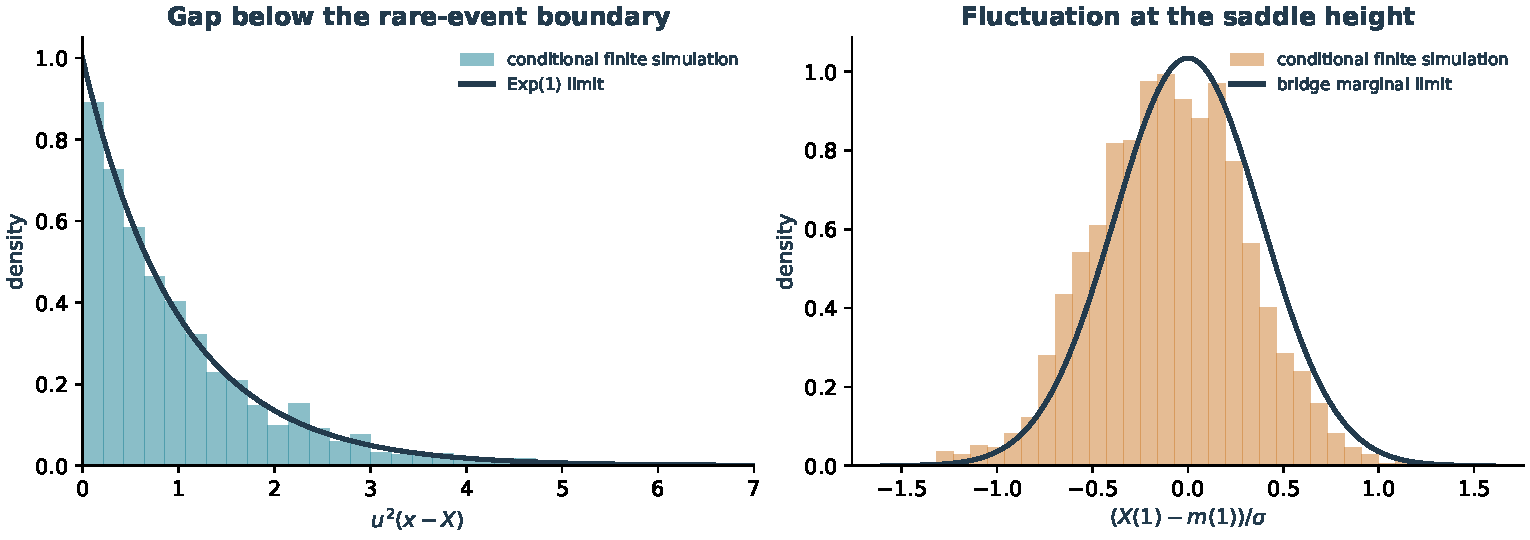
\includegraphics[width=\textwidth]{figures/finite_model_simulation.pdf}
 \caption{A finite synthetic-spectrum illustration at $u=128$.
 The solid curves are asymptotic limits, not fitted distributions.
 The data are not zeta-zero simulations.}
\end{figure}

These finite simulations do not establish asymptotic independence.
For example the correlation of the $c=2$ fluctuation with the boundary
slack is still approximately $-0.443$ at $u=128$. Such finite-saddle
effects remain visible and are reported in the raw data rather than
suppressed.

Third, a separate likelihood experiment compares the two independent
gamma products appearing in Theorem~\ref{mc:thm:threshold}. Its
synthetic points are
\[
 \widetilde\gamma_j=\frac{2\pi j}{W(j/e)},
\]
where $W$ is the principal Lambert function. They have the desired
Riemann--von Mangoldt counting asymptotic, but are not actual zeta
zeros. An exact likelihood-ratio event gives the Monte Carlo
total-variation estimate, using 50,000 draws for each row below.

\begin{table}[htbp]
\centering\small
\begin{tabular}{@{}rrrrrr@{}}
\toprule
$u$ & $c$ & Coordinates & TV estimate & Standard error & Limit in
\eqref{eq:overview-TV}\\
\midrule
1,000 & 1 & 62 & 0.04740 & 0.00095 & 0.06359\\
1,000 & 2 & 162 & 0.28110 & 0.00201 & 0.34826\\
1,000 & 3 & 277 & 0.67968 & 0.00209 & 0.78642\\
10,000 & 1 & 661 & 0.05080 & 0.00098 & 0.06359\\
10,000 & 2 & 1,546 & 0.30354 & 0.00206 & 0.34826\\
10,000 & 3 & 2,516 & 0.72354 & 0.00200 & 0.78642\\
\bottomrule
\end{tabular}
\caption{Finite product comparisons at
$h=c(u^4/\log u)^{1/5}$. The theorem does not supply a finite-$u$
error bound, and logarithmic convergence is slow.}
\end{table}

The differences from the limiting curve are appreciably larger than
Monte Carlo uncertainty. Even replacing the limiting parameter by
the exact finite sum $\tau_u^2$ need not eliminate the discrepancy:
at $(u,c)=(10{,}000,3)$ its Gaussian profile is about $0.73762$.
The numerical experiment illustrates the approach to the transition;
it is not a certified approximation for finite saddles.

\begin{figure}[htbp]
 \centering
 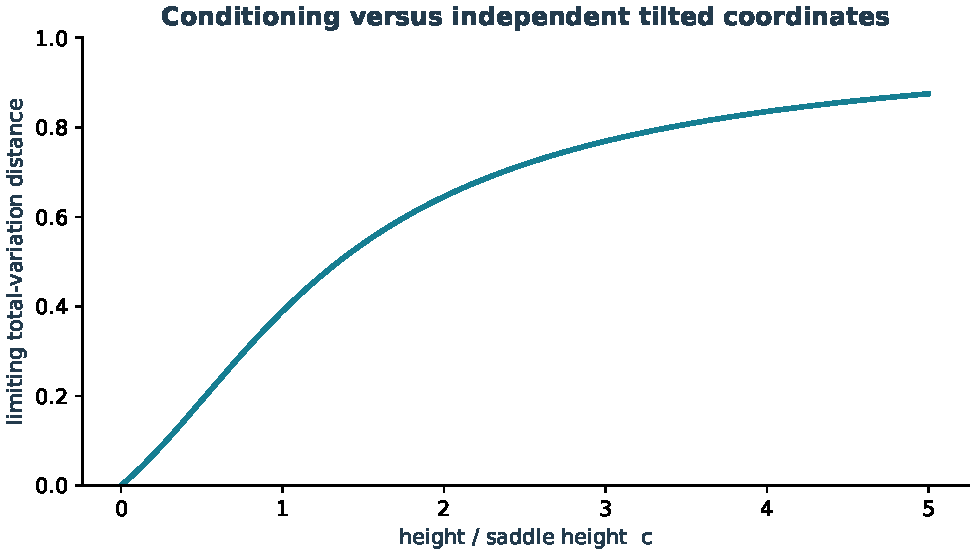
\includegraphics[width=0.78\textwidth]{figures/ensemble_transition.pdf}
 \caption{The separate transition for independence with the actual
unequal rates: the analytic function $D(V(c))$ from
Theorem~\ref{mc:thm:macroscopic}.}
\end{figure}

\subsection{Files and reproduction}

The archive contains this PDF, the complete \LaTeX{} sources, the
Python script, all figures in PDF/PNG format,
the numerical JSON output, source manifests, and review notes.
\path{README.md} explains the contents and commands;
\path{code/build_report.sh} rebuilds the PDF using \texttt{latexmk}.
The existing figures suffice to compile the manuscript, so rebuilding
it does not require repeating the simulation.

All conclusions concern explicitly defined random weights attached to
deterministic zero ordinates. They imply neither randomness of the
zeros nor a zero-spacing, pair-correlation, simplicity, or linear
independence theorem. Fixed conductors and fixed finite products are
allowed; no uniform result in a growing conductor or degree is claimed.
The general regular-variation theorem is unconditional. RH or
Dirichlet GRH supplies the exact completed-function interpretation
in the arithmetic applications.


\clearpage
\begin{thebibliography}{99}
\small
\raggedright
\addcontentsline{toc}{section}{References}

\bibitem{ProveItLean}
V. Reshetnikov, \emph{ProveIt: vendored grh-lean development}.
Snapshot \texttt{2a9f8e3ee74a1824d57546f0b1b4f1cef5df93d6},
inspected 27 November 2026.
\url{https://github.com/VladimirReshetnikov/ProveIt/tree/2a9f8e3ee74a1824d57546f0b1b4f1cef5df93d6/Analysis/GeneralizedRiemannHypothesis/vendor/grh-lean}.
Upstream: \url{https://github.com/lsernau/grh-lean}.

\bibitem{ProveItArticle}
V. Reshetnikov, \emph{ProveIt: Generalized Riemann Hypothesis,
Article}. Same pinned snapshot.
Section \texttt{ana:sec:smalldev}, results
\texttt{ana:thm:gammasum} and \texttt{ana:thm:smalldev}.
\url{https://github.com/VladimirReshetnikov/ProveIt/tree/2a9f8e3ee74a1824d57546f0b1b4f1cef5df93d6/Analysis/GeneralizedRiemannHypothesis/Article}.

\bibitem{Sutherland}
A. V. Sutherland, \emph{Independent verification of the Lean
formalization of RH and GRH}, verification page, accessed
27 November 2026.
\url{https://klein.mit.edu/~drew/shortgrh/}.

\bibitem{RoynetteYor}
B. Roynette and M. Yor, Couples de Wald ind\'efiniment divisibles.
Exemples li\'es \`a la fonction gamma d'Euler et \`a la fonction zeta
de Riemann, \emph{Annales de l'Institut Fourier} \textbf{55} (2005),
no.~4, 1219--1283.
\url{https://doi.org/10.5802/aif.2125}.

\bibitem{GaoHannigLeeTorcaso}
F. Gao, J. Hannig, T.-Y. Lee, and F. Torcaso,
Laplace transforms via Hadamard factorization,
\emph{Electronic Journal of Probability} \textbf{8} (2003),
paper no.~13, 1--20.
\url{https://doi.org/10.1214/EJP.v8-151}.

\bibitem{CampenhoutCover}
J. M. Van Campenhout and T. M. Cover,
Maximum entropy and conditional probability,
\emph{IEEE Transactions on Information Theory} \textbf{27} (1981),
no.~4, 483--489.
\url{https://isl.stanford.edu/people/cover/papers/transIT/0483camp.pdf}.

\bibitem{MayerWolfZeitouni}
E. Mayer-Wolf and O. Zeitouni,
The probability of small Gaussian ellipsoids and associated conditional
moments, \emph{Annals of Probability} \textbf{21} (1993), no.~1, 14--24.
\url{https://www.wisdom.weizmann.ac.il/~zeitouni/pdf/eddyelip.pdf}.

\bibitem{SobolevShklyaev}
I. V. Sobolev and A. V. Shklyaev,
Large deviations of weighted sums of independent identically distributed
random variables with functionally-defined weights,
\emph{Fundamentalnaya i Prikladnaya Matematika} \textbf{23} (2020),
no.~1, 191--206; English translation,
\emph{Journal of Mathematical Sciences} \textbf{262} (2022),
no.~4, 525--536.
\url{https://www.mathnet.ru/eng/fpm1874}.

\bibitem{Sra}
S. Sra, \emph{On some positivity properties of the Riemann Xi
function}, version 3, 2 November 2026, especially Appendix C.17.
\url{https://suvrit.github.io/papers/riem-xi/riem-xi-v3.pdf}.

\bibitem{BennettEtAl}
M. A. Bennett, G. Martin, K. O'Bryant, and A. Rechnitzer,
Counting zeros of Dirichlet $L$-functions,
\emph{Mathematics of Computation} \textbf{90} (2021), no.~329,
1455--1482.
\url{https://doi.org/10.1090/mcom/3599}.
Preprint: \url{https://arxiv.org/abs/2005.02989}.

\end{thebibliography}

\end{document}
